\documentclass{article}
\usepackage{stackengine}
%\usepackage[utf8]{inputenc}
\usepackage[T1]{fontenc}
\usepackage{amsmath}
\usepackage{amsfonts}
\usepackage{graphicx}
\usepackage{pbsi}
\usepackage{lmodern}
%\usepackage{tgbonum}
%\usepackage[a5paper]{geometry}
\usepackage{pdflscape}
\usepackage[dvipsnames, svgnames]{xcolor}
\usepackage[pages=some]{background}
\usepackage{tikz}
\usetikzlibrary{math} 
\usetikzlibrary{automata,positioning}
\usetikzlibrary[decorations.text]

%\usetikzlibrary[automata]

\usetikzlibrary{calc}
\newcommand*{\vertchar}[2][0pt]{%
  \tikz[
    inner sep=1pt,
    shorten >=-.15ex,
    shorten <=-.15ex,
    line cap=round,
    baseline=(c.base),
  ]\draw
    (0,0) node (c) {#2}
    ($(c.north)+(#1,0)$) -- ($(c.north)+(#1,0)$);%
}


\makeatletter
\newcommand{\dotr}[1]{%
  \mathpalette\@dotr{#1}%
}

\newcommand*{\@dotr}[2]{%
  % #1: math style (\displaystyle, ..., \scriptscriptstyle)
  % #2: argument of \dotr
  \sbox0{$\m@th#1#2$}%
  \usebox{0}%
  % simulating a superscript
  %\raisebox{\dimexpr\ht0-\height}{$\m@th#1\addvbuffer[-1ex 0.9ex]{.}}%
  \raisebox{3.5pt}{$\m@th#1\@smallbullet#1\bullet$}%
  \kern\scriptspace
}
\newcommand*{\@smallbullet}[2]{%
  \scalebox{.3}{$\m@th#1#2$}%
}
\makeatother
    
\newcommand*{\siin}[1]{\stackinset{c}{}{b}{5.5pt}{\small\ttfamily\char'15}{#1}}
\newcommand*{\nn}{\textsuperscript{n}}

\newcommand*{\pehin}[1]{\stackinset{c}{}{b}{5.5pt}{\small\ttfamily\char'15}{#1}}
\newcommand*{\dtr}{\raisebox{3.5pt}{$\scalebox{.3}{$\bullet$}$}}
\newcommand*{\dtrh}{\raisebox{5pt}{$\scalebox{.3}{$\bullet$}$}}



\begin{document}

\hspace*{-30mm}
\resizebox{18cm}{!} {
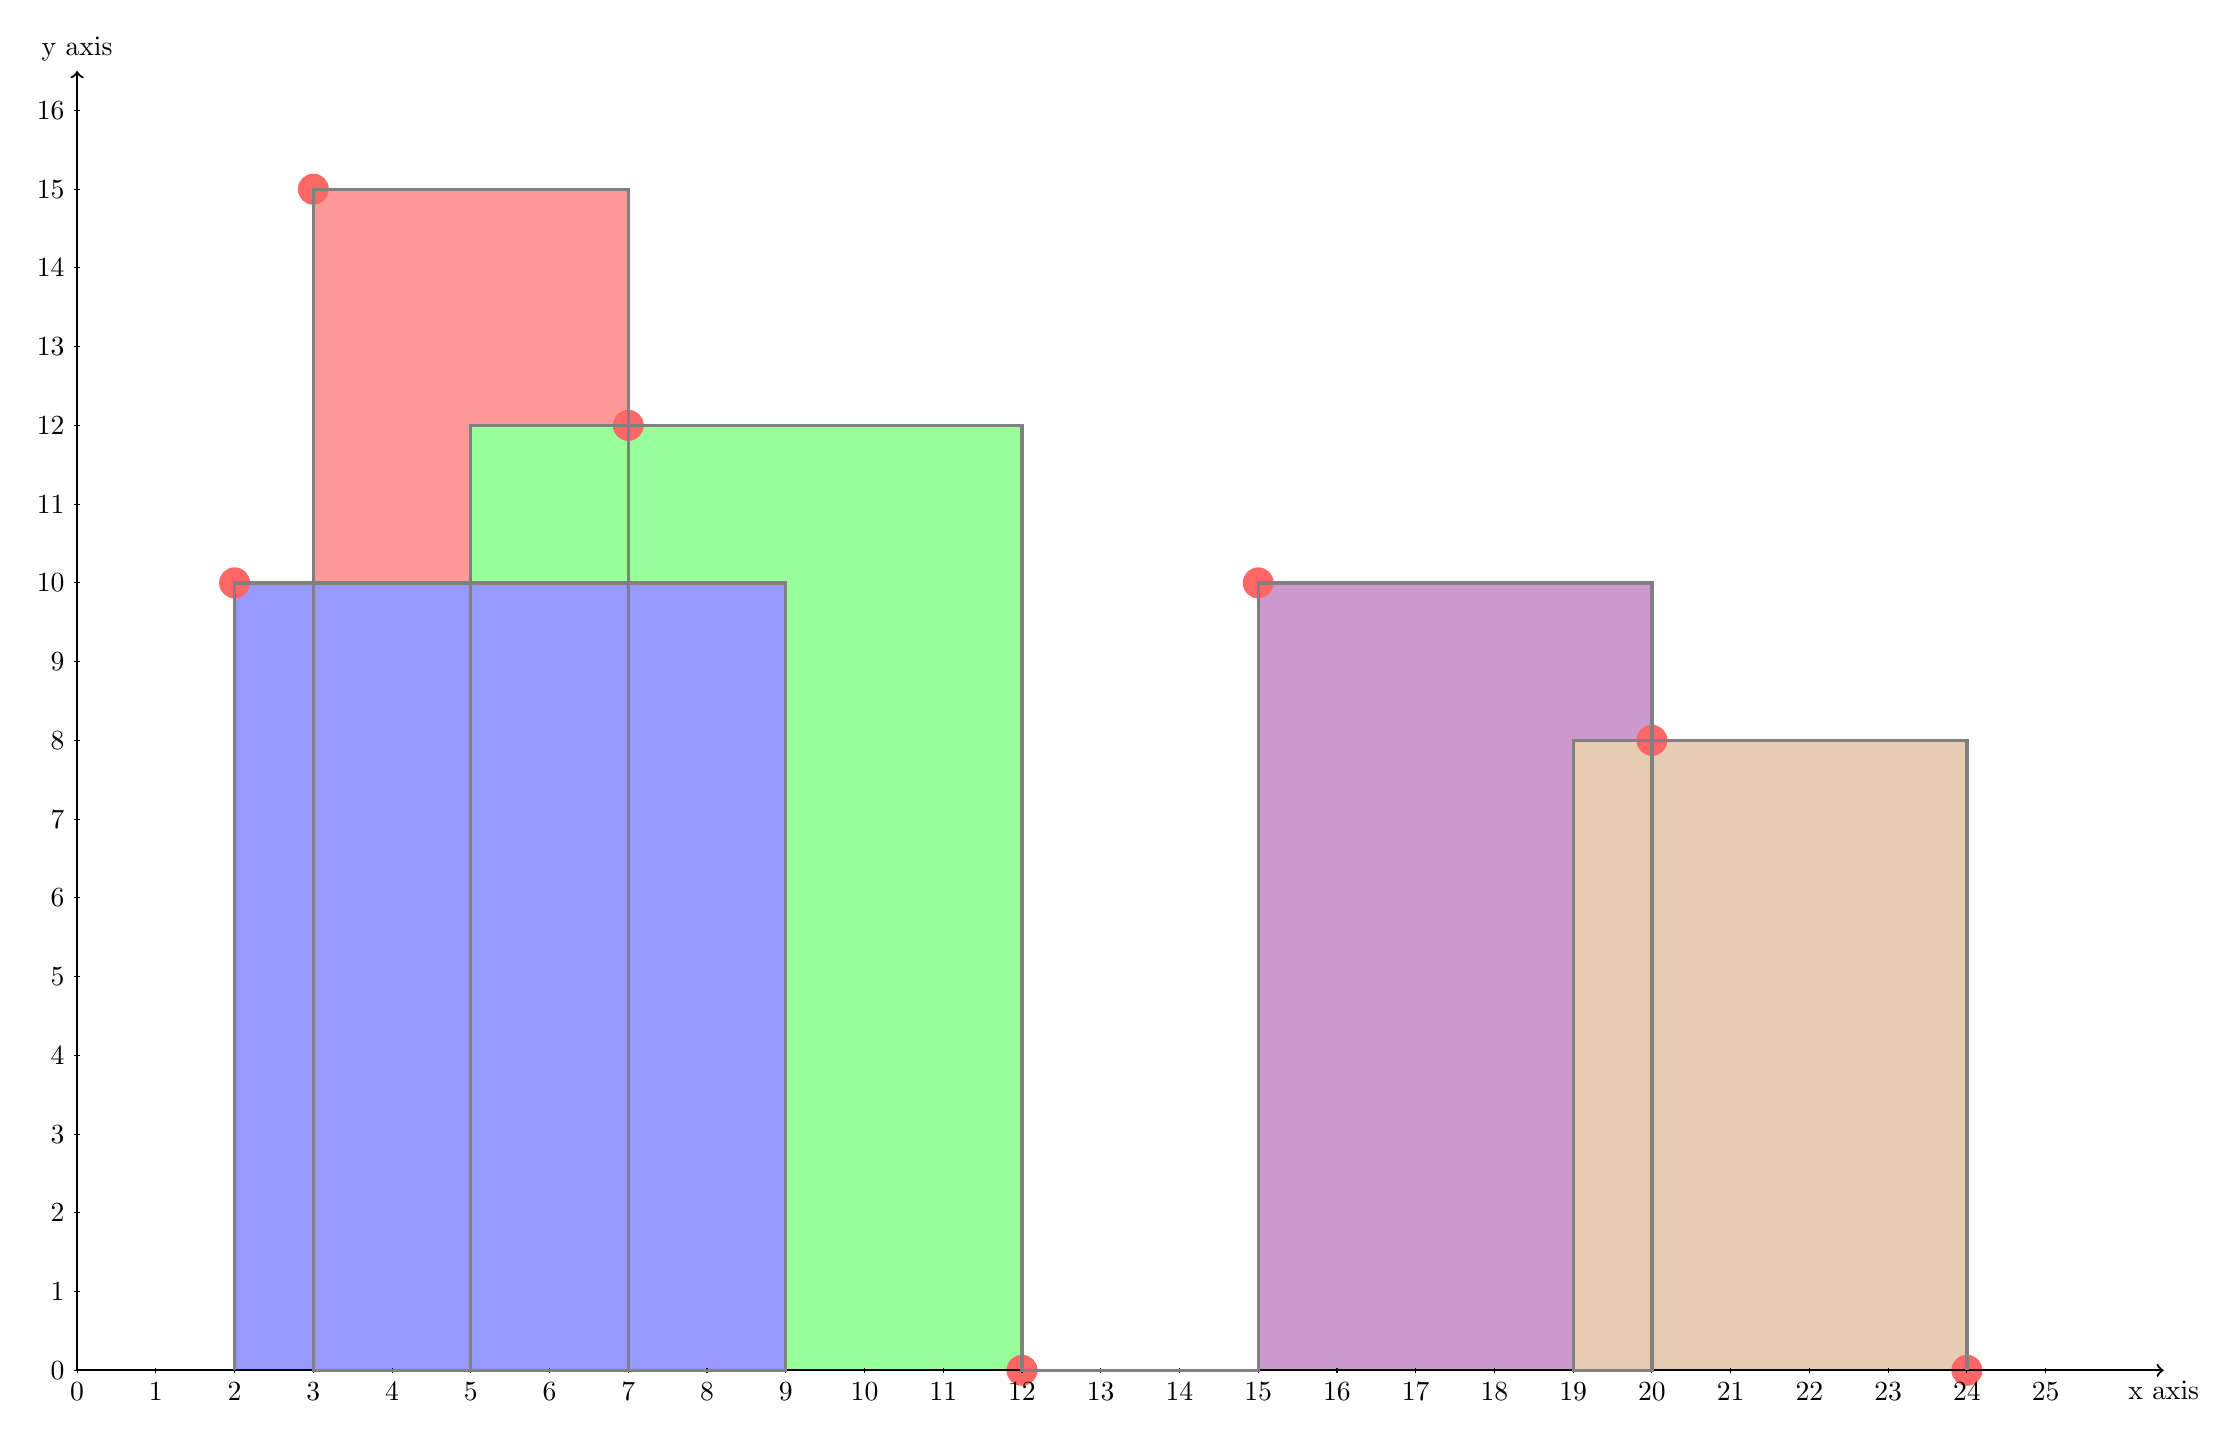
\begin{tikzpicture} 
%\draw [help lines] grid (4,4); 
%\draw[step=1cm,gray,very thin] (0,0) grid (25,16);
%\draw [red, dashed, very thick] (0,0) -- (2,0) (0,1) -- (2,1);
\filldraw[fill=red!40!white, draw=black] (3,0) rectangle (7,15);
\filldraw[fill=green!40!white, draw=black] (5,0) rectangle (12,12);
\filldraw[fill=blue!40!white, draw=black] (2,0) rectangle (9,10);
\filldraw[fill=violet!40!white, draw=black] (15,0) rectangle (20,10);
\filldraw[fill=brown!40!white, draw=black] (19,0) rectangle (24,8);
\filldraw[color=red!60!white, fill=red!60!white, very thick] (2,10) circle (5pt);
\filldraw[color=red!60!white, fill=red!60!white, very thick] (3,15) circle (5pt);
\filldraw[color=red!60!white, fill=red!60!white, very thick] (7,12) circle (5pt);
\filldraw[color=red!60!white, fill=red!60!white, very thick] (12,0) circle (5pt);
\filldraw[color=red!60!white, fill=red!60!white, very thick] (15,10) circle (5pt);
\filldraw[color=red!60!white, fill=red!60!white, very thick] (20,8) circle (5pt);
\filldraw[color=red!60!white, fill=red!60!white, very thick] (24,0) circle (5pt);


%\draw[thick,->] (0,0) -- (26,0);
%\draw[thick,->] (0,0) -- (0,16);
\foreach \x in {0,1,2,3,4,5,6,7,8,9,10,11,12,13,14,15,16,17,18,19,20,21,22,23,24,25}
   \draw (\x cm,1pt) -- (\x cm,-1pt) node[anchor=north] {$\x$};
\foreach \y in {0,1,2,3,4,5,6,7,8,9,10,11,12,13,14,15,16}
    \draw (1pt,\y cm) -- (-1pt,\y cm) node[anchor=east] {$\y$};
\draw[thick,->] (0,0) -- (26.5,0) node [anchor= north]{x axis};
\draw[thick,->] (0,0) -- (0,16.5) node [anchor= south] {y axis};


\draw [gray, very thick] (2,0) -- (2,10) -- (9,10) -- (9,0) -- (3,0) -- (3,15) -- (7,15) -- (7,0) -- (5,0) -- (5,12) -- (12,12) -- (12,0) -- (15,0) -- (15,10) -- (20,10) -- (20,0) -- (19,0) -- (19,8) -- (24,8) -- (24,0);
\end{tikzpicture}
}

\end{document}